\documentclass[10pt,leter,openany]{article}
\usepackage[latin1]{inputenc}
\usepackage[english]{babel}
\usepackage{amsmath}
\usepackage{amsfonts}
\usepackage{amssymb}
\usepackage{graphicx}
\usepackage{listings}
\usepackage{color}
\usepackage[left=3cm,right=3cm,top=3cm,bottom=3cm]{geometry}
\usepackage[numbers,sort&compress]{natbib}
\usepackage{url}
\usepackage{caption}
\usepackage{siunitx}
%\usepackage{subfigure}
\usepackage{float}
\usepackage{booktabs}
\usepackage{subcaption}
\usepackage{comment}
\usepackage{mwe}
%\usepackage[table,xcdraw]{xcolor}
\usepackage[shortlabels]{enumitem}   %To enumerate with letters
\usepackage{mathtools}	%To write derivates
\usepackage[thinc]{esdiff}	%To write derivates
\usepackage{cancel} %To cancel terms in equations

\setlength{\parindent}{0pt}
\setlength{\parskip}{4pt}

\definecolor{mygreen}{rgb}{0,0.6,0}
\definecolor{mygray}{rgb}{0.5,0.5,0.5}
\definecolor{mymauve}{rgb}{0.58,0,0.82}

\lstset{ 
	backgroundcolor=\color{white},   % choose the background color; you must add \usepackage{color} or \usepackage{xcolor}; should come as last argument
	basicstyle=\footnotesize,        % the size of the fonts that are used for the code
	breakatwhitespace=false,         % sets if automatic breaks should only happen at whitespace
	breaklines=true,                 % sets automatic line breaking
	captionpos=b,                    % sets the caption-position to bottom
	commentstyle=\color{mygreen},    % comment style
	deletekeywords={...},            % if you want to delete keywords from the given language
	escapeinside={\%*}{*)},          % if you want to add LaTeX within your code
	extendedchars=true,              % lets you use non-ASCII characters; for 8-bits encodings only, does not work with UTF-8
	firstnumber=01,                	 % start line enumeration with line 1000
	frame=single,	                 % adds a frame around the code
	keepspaces=true,                 % keeps spaces in text, useful for keeping indentation of code (possibly needs columns=flexible)
	keywordstyle=\color{blue},       % keyword style
	language=Python,                 % the language of the code
	morekeywords={*,...},            % if you want to add more keywords to the set
	numbers=left,                    % where to put the line-numbers; possible values are (none, left, right)
	numbersep=5pt,                   % how far the line-numbers are from the code
	numberstyle=\tiny\color{mygray}, % the style that is used for the line-numbers
	rulecolor=\color{black},         % if not set, the frame-color may be changed on line-breaks within not-black text (e.g. comments (green here))
	showspaces=false,                % show spaces everywhere adding particular underscores; it overrides 'showstringspaces'
	showstringspaces=false,          % underline spaces within strings only
	showtabs=false,                  % show tabs within strings adding particular underscores
	stepnumber=1,                    % the step between two line-numbers. If it's 1, each line will be numbered
	stringstyle=\color{mymauve},     % string literal style
	tabsize=2,	                     % sets default tabsize to 2 spaces
	title=\lstname                   % show the filename of files included with \lstinputlisting; also try caption instead of title
}

\usepackage[dvipsnames,table,xcdraw]{xcolor}

\usepackage{fancyvrb}

% redefine \VerbatimInput
\RecustomVerbatimCommand{\VerbatimInput}{VerbatimInput}%
{fontsize=\footnotesize,
	%
	frame=lines,  % top and bottom rule only
	framesep=2em, % separation between frame and text
	rulecolor=\color{Gray},
	%
	label=\fbox{\color{Black}data.txt},
	labelposition=topline,
	%
	commandchars=\|\(\), % escape character and argument delimiters for
	% commands within the verbatim
	commentchar=*        % comment character
}



\usepackage{titling}
\newcommand{\subtitle}[1]{%
	\posttitle{%
		\par\end{center}
	\begin{center}\large#1\end{center}
	\vskip0.5em}%
}


\author{5273}
\title{Homework Assignment 11: Applied Probabilistic Models}
\subtitle{Multivariate distributions and probability densities}
\date{}


\begin{document}
	
\maketitle

\section{Introduction}
 	For this work aspects of multivariate probability densities and distribution are discussed. To begin with, a convolution of distribution example is performed, in the area of finance, specifically in stock prices of two companies. As a second point, a Chi-squared test is performed for two categorical variables in the analysis of the results of my thesis work \citep{hernandez2020study}. Finally, a numerical covariance analysis is performed, in order to prove two properties of this statistical value, also with prices on the stock market between two other enterprises.
 	
 	For the analysis, the R software is used in its version 4.0.2 \citep{r}, and the code used is available on the GitHub repository \citep{github}. This work is run on a MacBook Air with an Intel Core i5 CPU $ @ $ 1.8 GHz and 8 GB RAM.

\section{Convolution of Distributions}
	 This section is about the convolution of probability distributions. The convolution can be considered as the operation of forming linear combinations of random variables. Then, the probability density function (PDF) of a sum of random variables is the convolution of their corresponding PDF. This sum, let be $ Z = X + Y$, for example, of two random variables, can be expressed as mentioned in Equation \ref{eq:convolution_discrete} for discrete variables and Equation \ref {eq:convolution_continuous} for continuous ones.
		\begin{equation} \label{eq:convolution_discrete}
			P(Z=z) = \displaystyle\sum_{k=-\infty}^{\infty} P(X=k)P(Y=z-k)
		\end{equation}
	
		\begin{equation} \label{eq:convolution_continuous}
			h(z) = (f*g)(z) = \displaystyle \int_{-\infty}^{\infty}f(z-t)g(t)dt = \displaystyle\int_{-\infty}^{\infty}f(t)g(z-t)dt
		\end{equation}
	For the convolution example data are downloaded from Yahoo! Finance \citep{yahoo}, corresponding to the values of the stock prices of Amazon and Tesla Motors enterprises, which correspond to the timeframe of September 2019 - September 2020. The data used for the analysis is the adjusted close price of the stock, which is the closing price after adjustments for all applicable splits and dividend distributions.  It includes trading days only, which means that Saturdays, Sundays, and national holidays are not quoted as the stock market is not open on those days. Figure \ref{fig:box1} and Figure \ref{fig:dens1} show a boxplot and density plot respectively created to represent differences of the data. Then, Figure \ref{fig:conv1} shows a histogram of the convolution of the distributions.
	
		\begin{figure}
			\begin{center}
				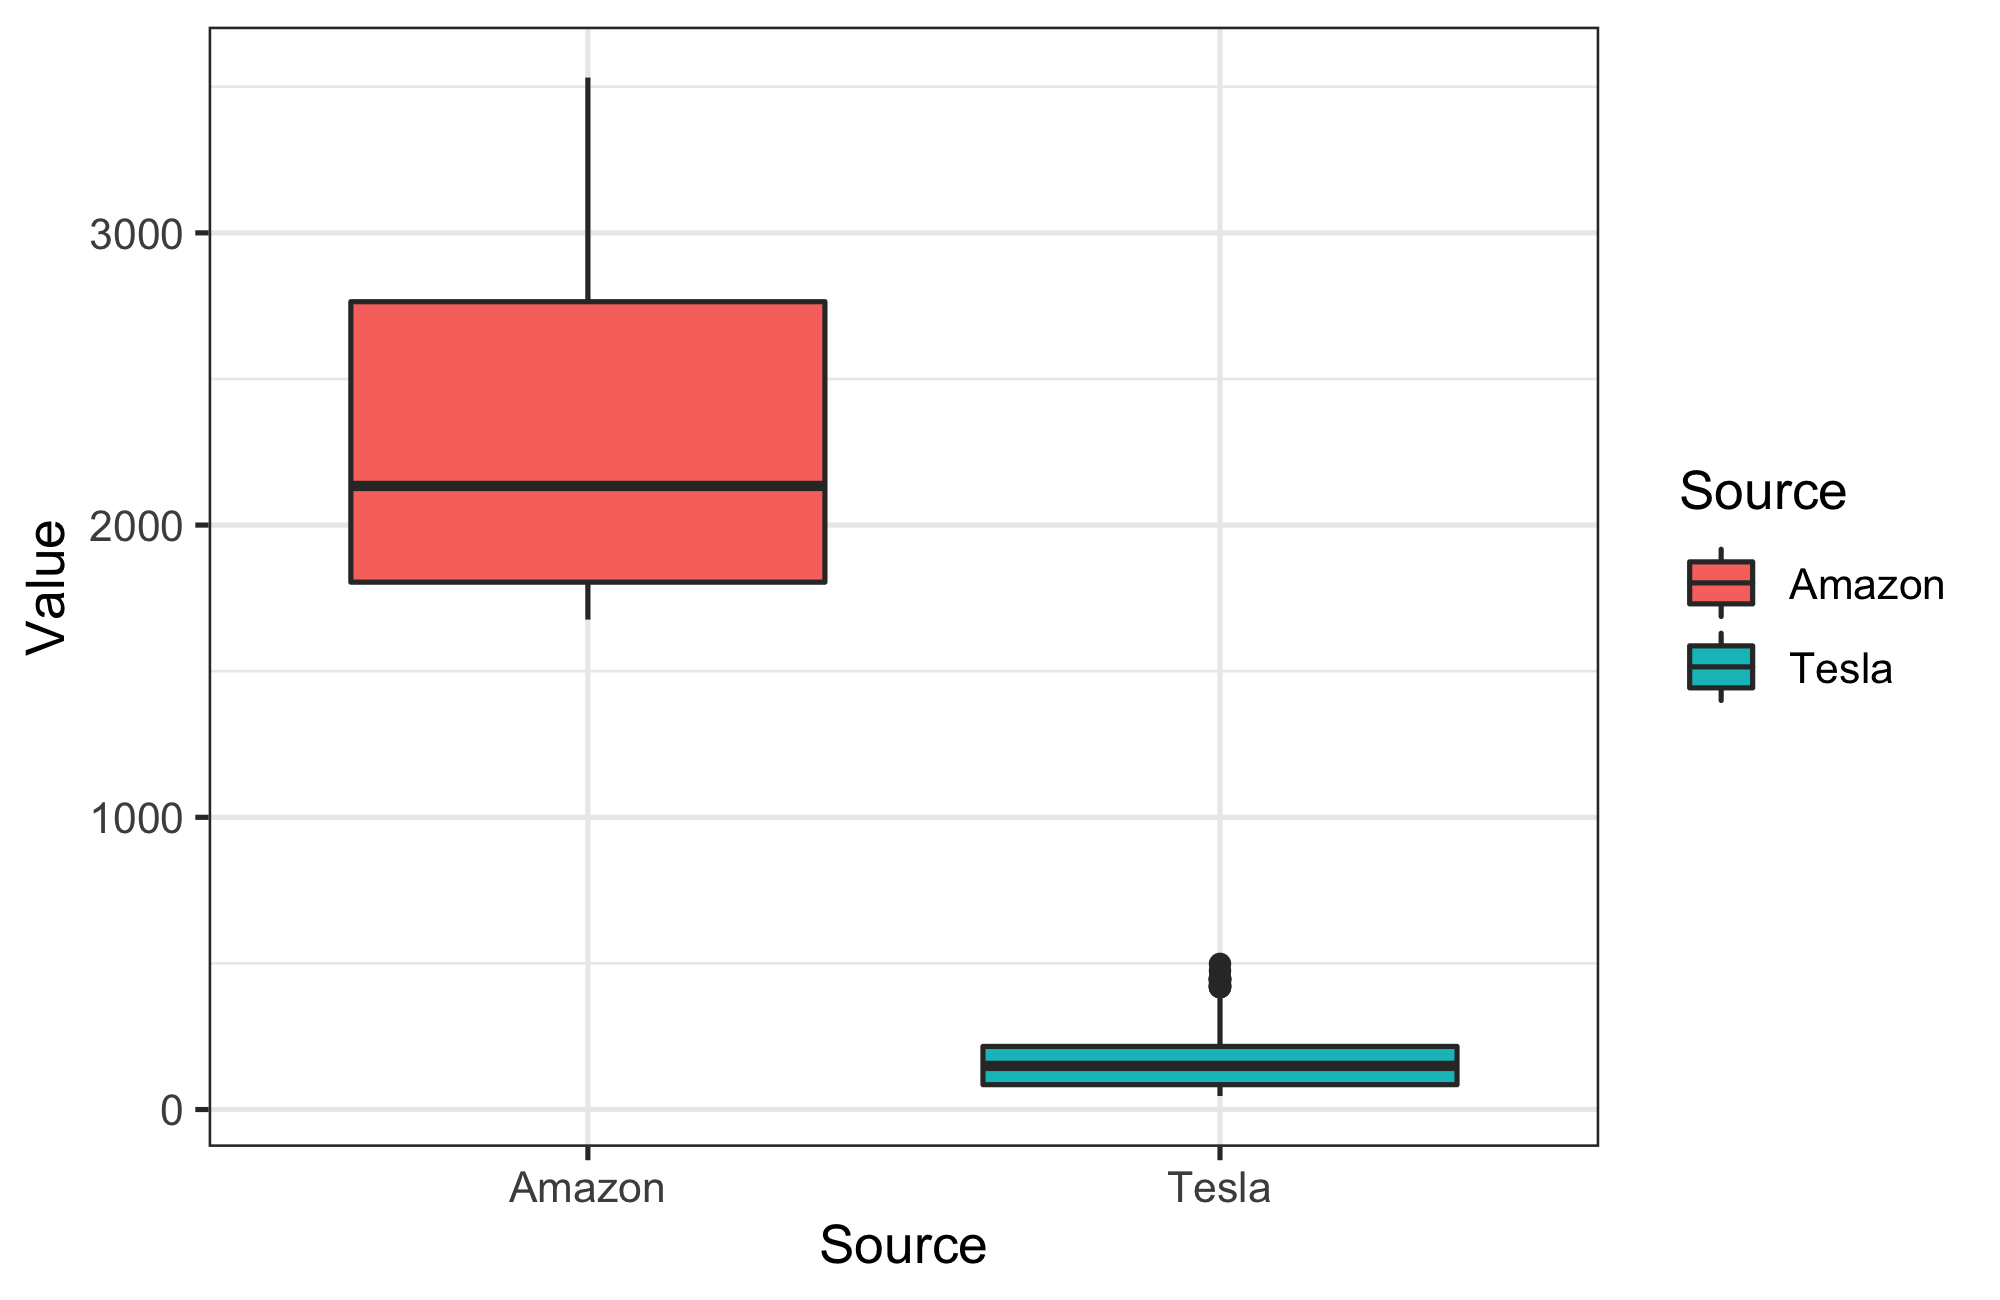
\includegraphics[scale=0.21]{extras/boxplot_stocks}
				\captionof{figure}{Boxplots of the Adjusted Close Price of Amazon and Tesla }
				\label{fig:box1}
			\end{center}
		\end{figure}

		\begin{figure}
			\begin{center}
				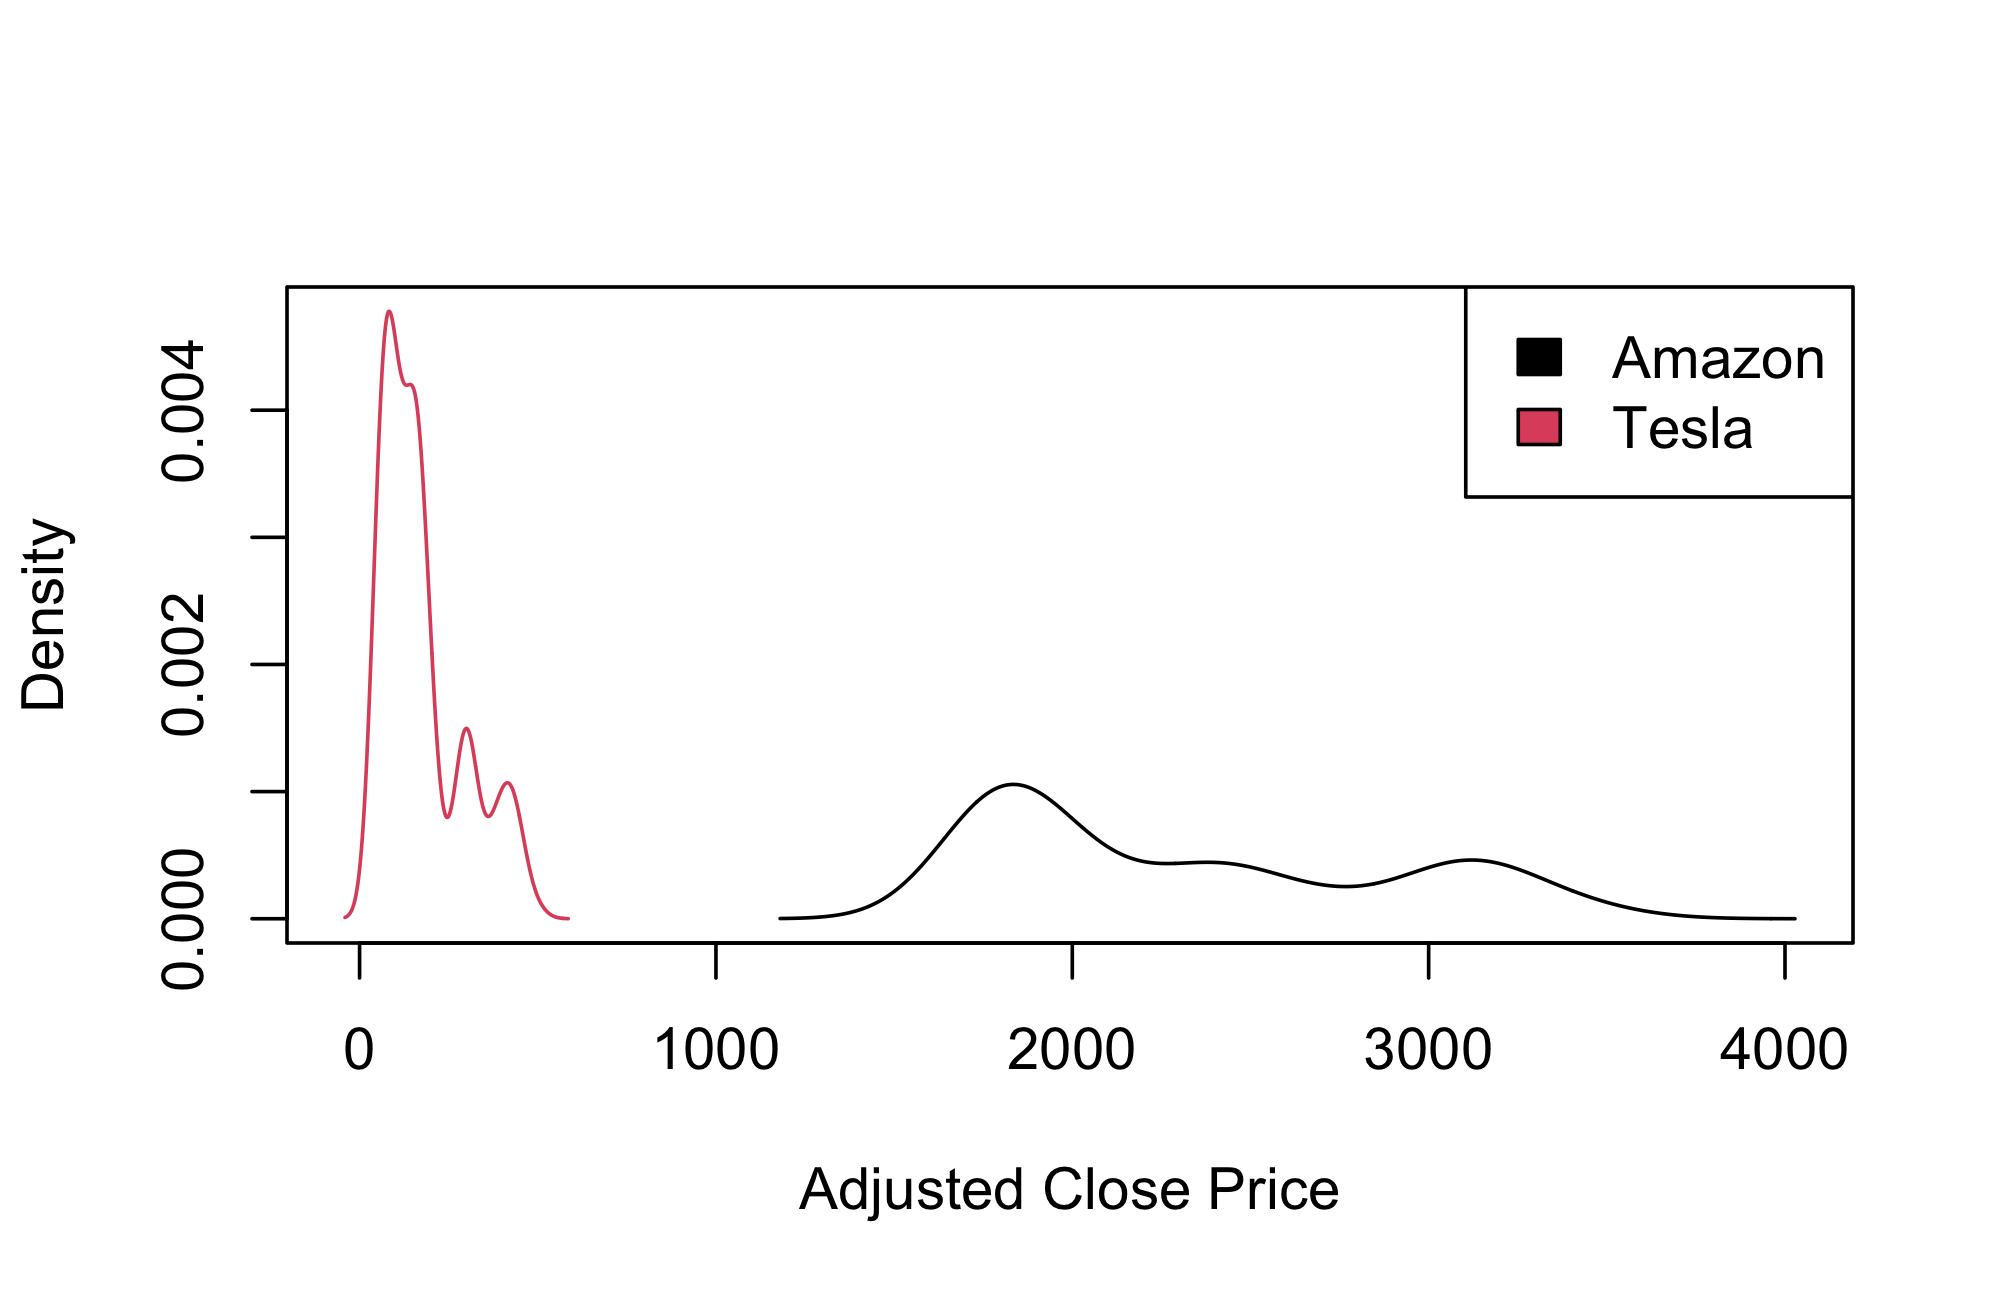
\includegraphics[scale=0.21]{extras/dens}
				\captionof{figure}{Densplot of the Adjusted Close Price of Amazon and Tesla }
				\label{fig:dens1}
			\end{center}
		\end{figure}
		
		\begin{figure}
			\begin{center}
				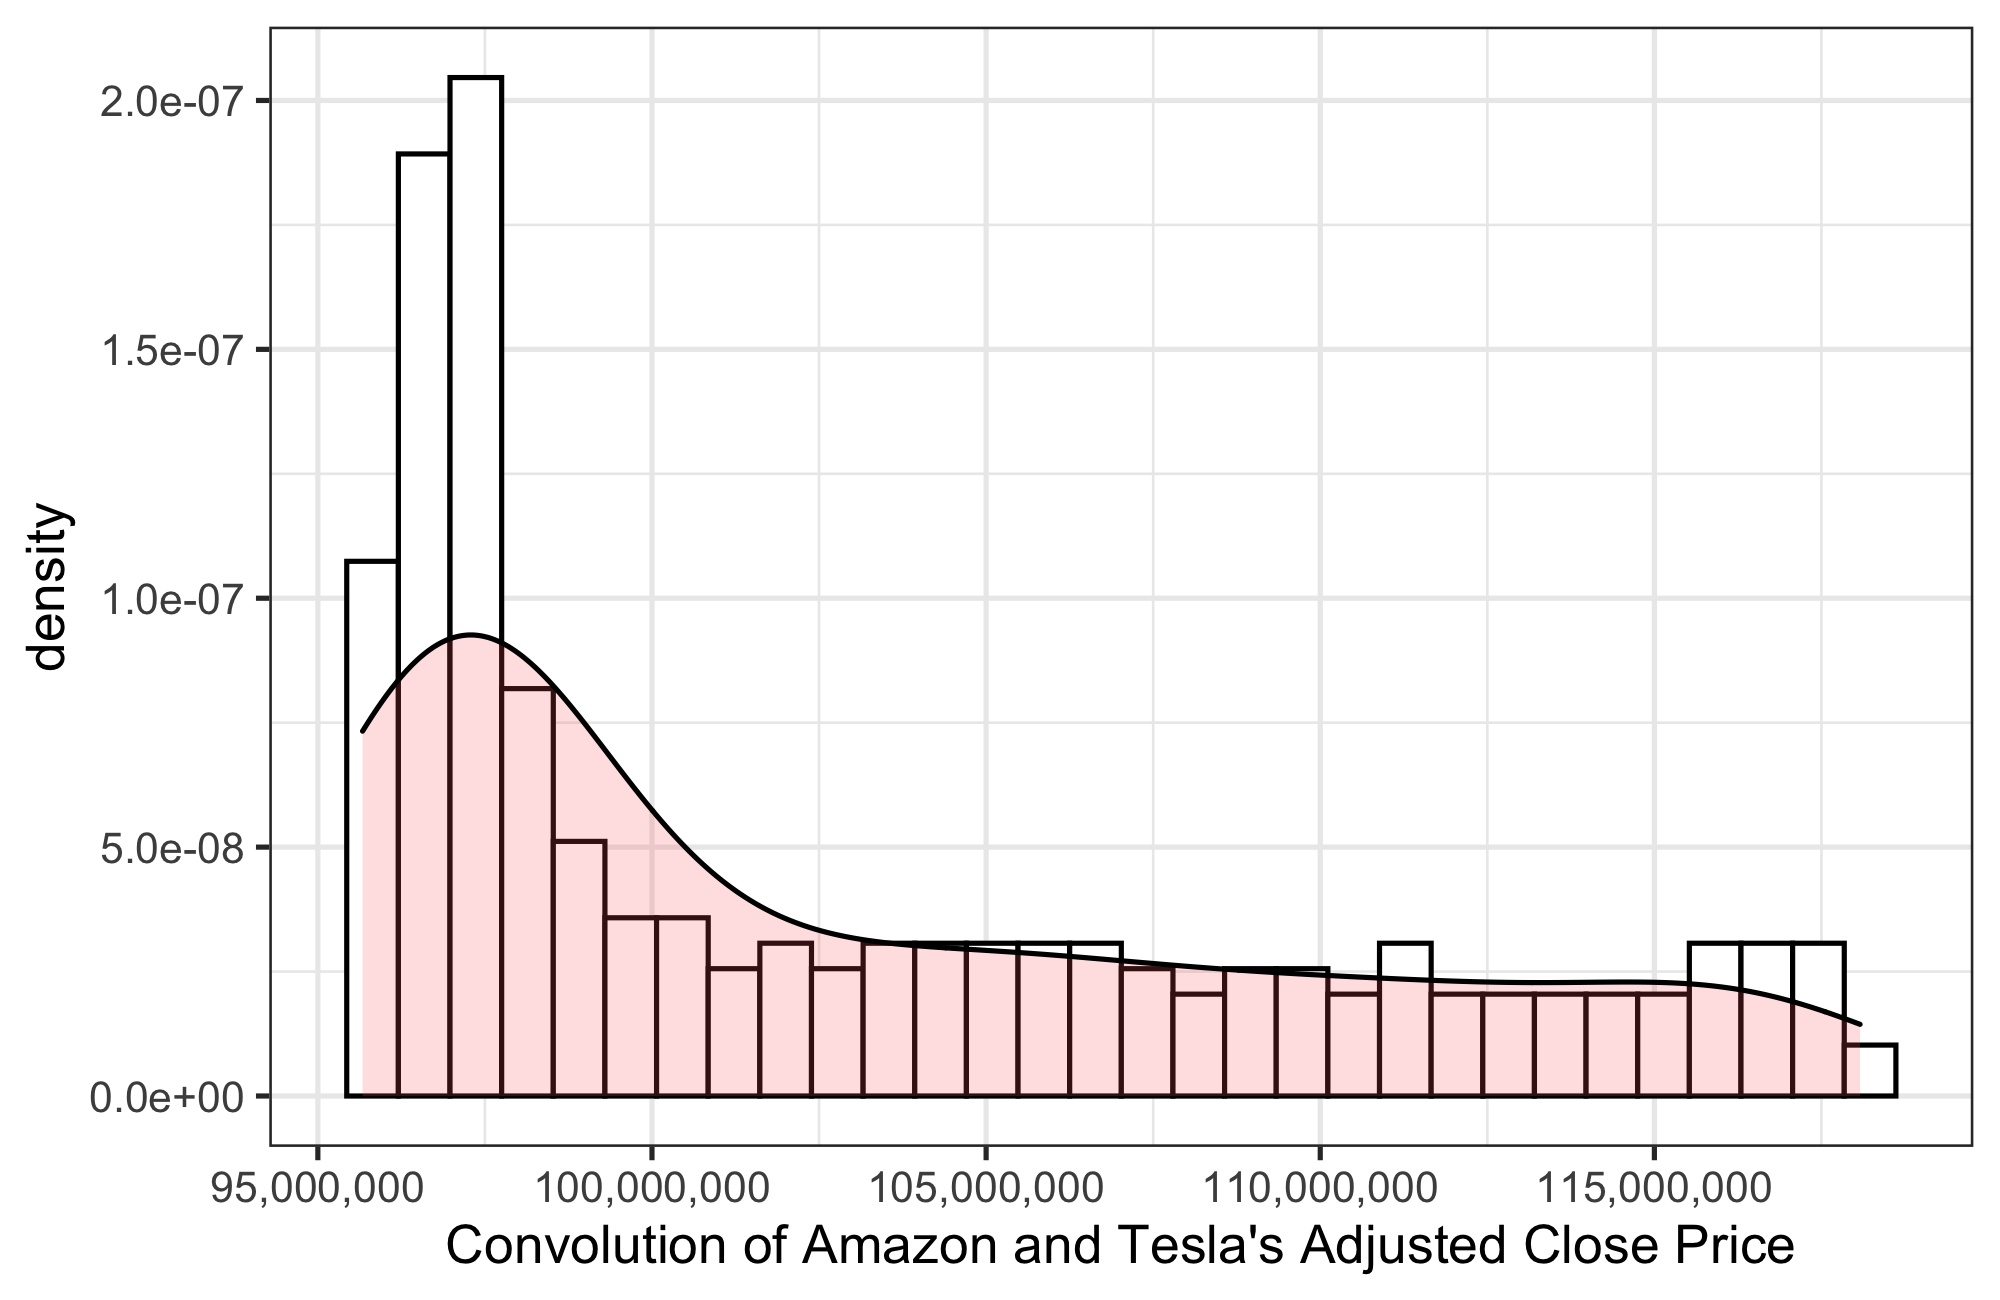
\includegraphics[scale=0.21]{extras/hist_stocks}
				\captionof{figure}{Histogram of the Convolution of the Adjusted Close Price of Amazon and Tesla }
				\label{fig:conv1}
			\end{center}
		\end{figure}


\section{Chi-Squared Test}

The Chi-Square Test of independence tests whether there is a relationship between two or more categorical variables  \citep{soetewey2020}.  Categorical or nominal data refers that one uses labels instead of numbers; for example race and gender are categorical variables. The central tendency of categorical variables is given by its mode, since median and mean can only be computed on numerical data. Therefore, it does not follow a normal bell-curve distribution, and cannot be analyzed with tests based on a normal distribution such as the $t$-test or ANOVA. The hypotheses are:
\begin{itemize}
	\item $H_{0}$: The variables are independent there is no relationship between the two categorical variables. Knowing the value of one variable does not help to predict the value of the other variable.
	\item $H_{1}$: The variables are dependent, there is a relationship between the two categorical variables. Knowing the value of one variable helps to predict the value of the other variable.
\end{itemize}

To perform the test, data are taken from the results of my thesis work. For this example,\textit{Dataset} and \textit{Optimal} are the two categorical variables which are the ones to be analyzed. Figure \ref{fig:pies} shows how instances performed with these variables. Besides, a contingency table analysis is performed, which is shown below. The hypothesis to be tested is that Dataset and Optimal are not associated with one another. The $p$-value is $1.33 \times 10^{-7}$, which is less than the significance level of 0.05, so the null hypothesis is rejected, and the conclusion from this hypothesis test is that the dataset and optimal values are not independent, therefore are associated somehow. Finally, the last contingency table contains the expected values which would be true the null hypothesis.
		 \begin{figure}
			\centering
			\begin{subfigure}[b]{0.475\textwidth}
				\centering
				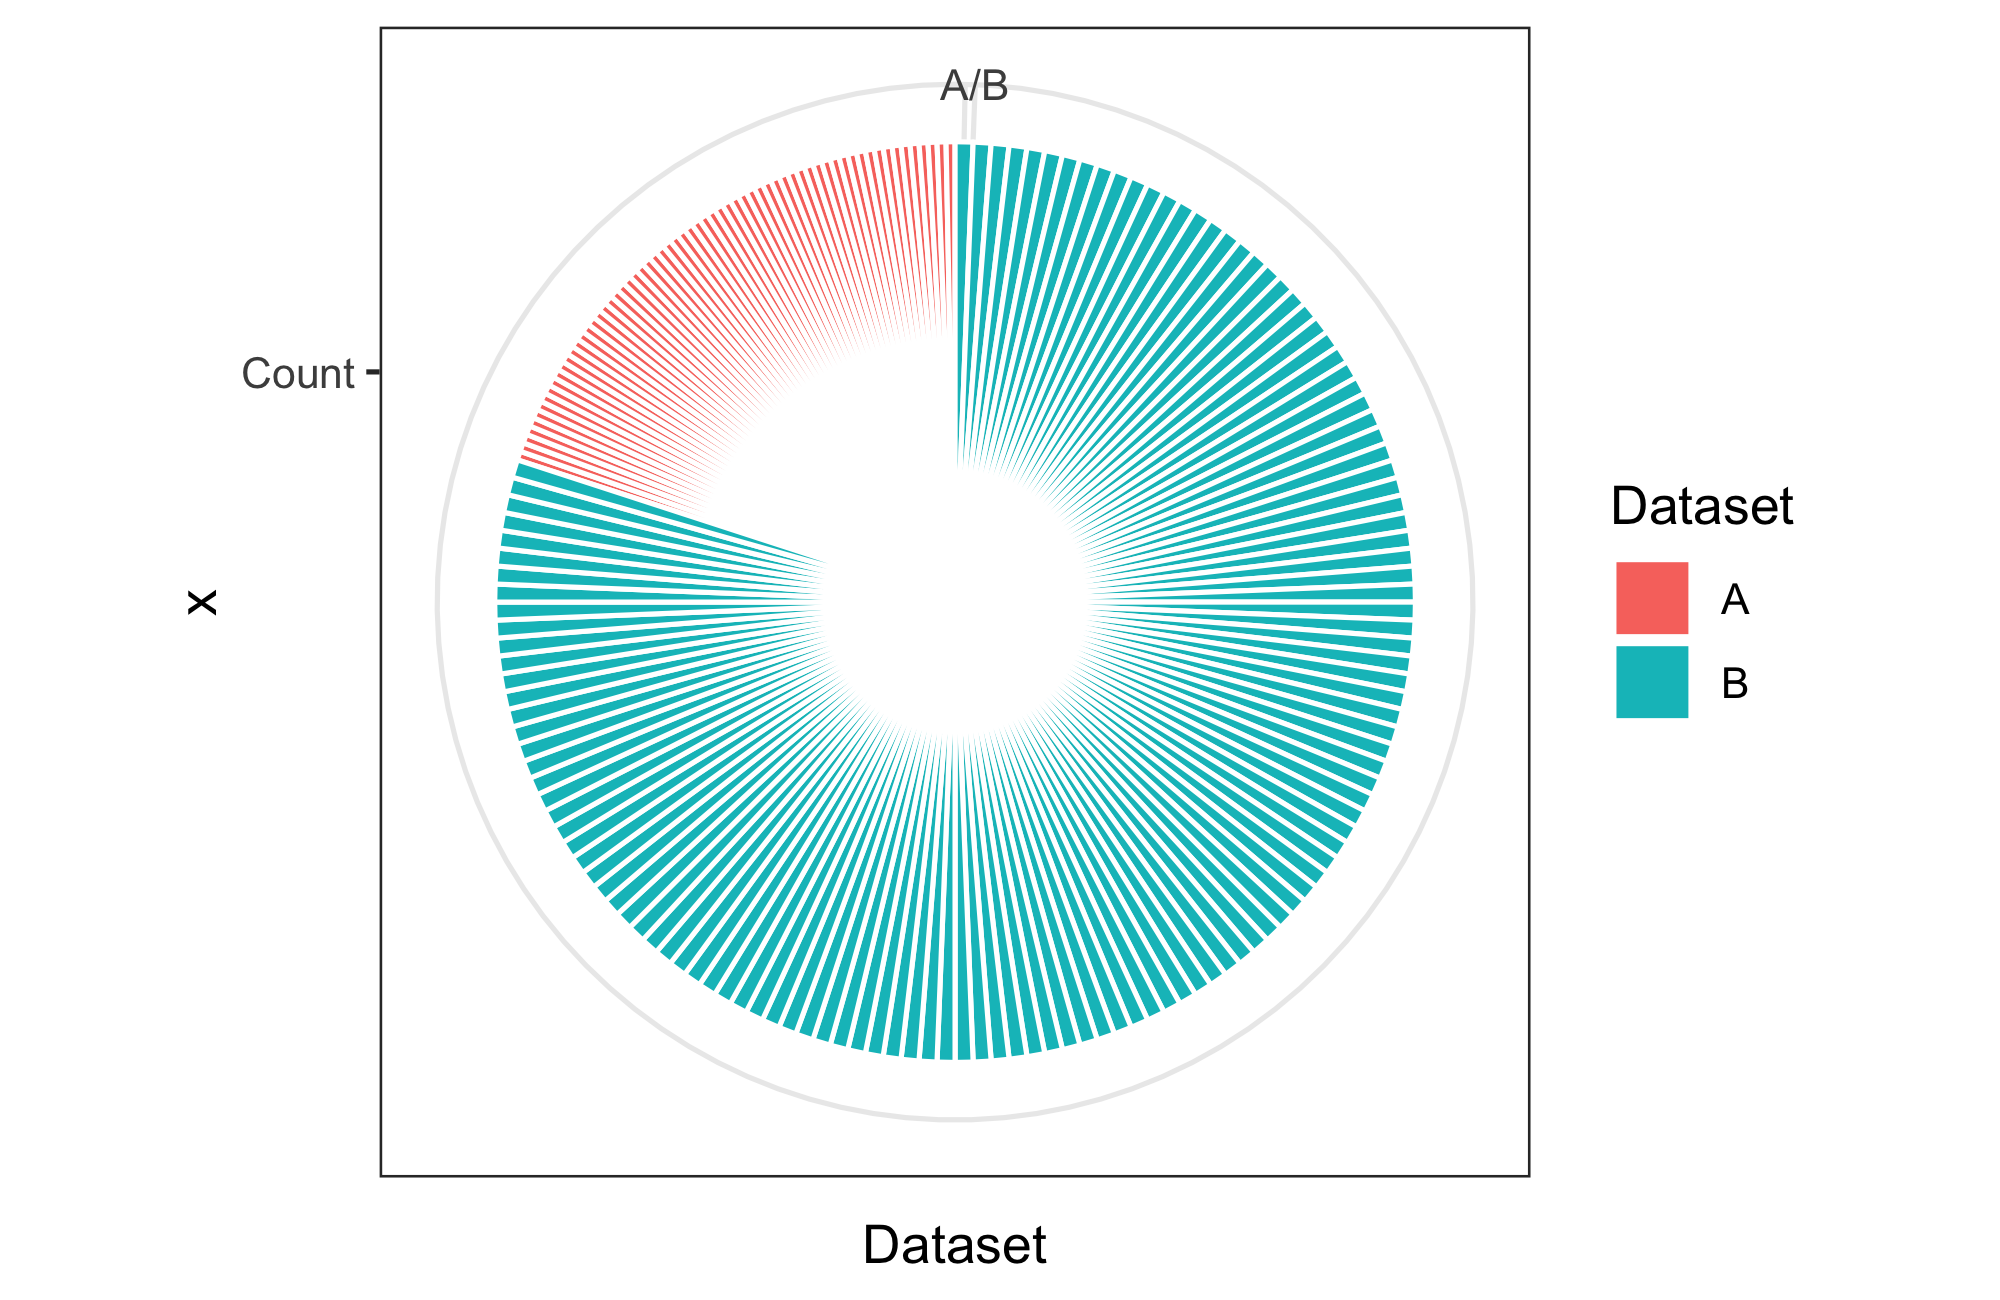
\includegraphics[width=\textwidth]{extras/pie_dataset}
				\caption[]%
				{{\small Groups of data of Instances}}    
				\label{fig:pie_dataset}
			\end{subfigure}
			\hfill
			\begin{subfigure}[b]{0.475\textwidth}  
				\centering 
				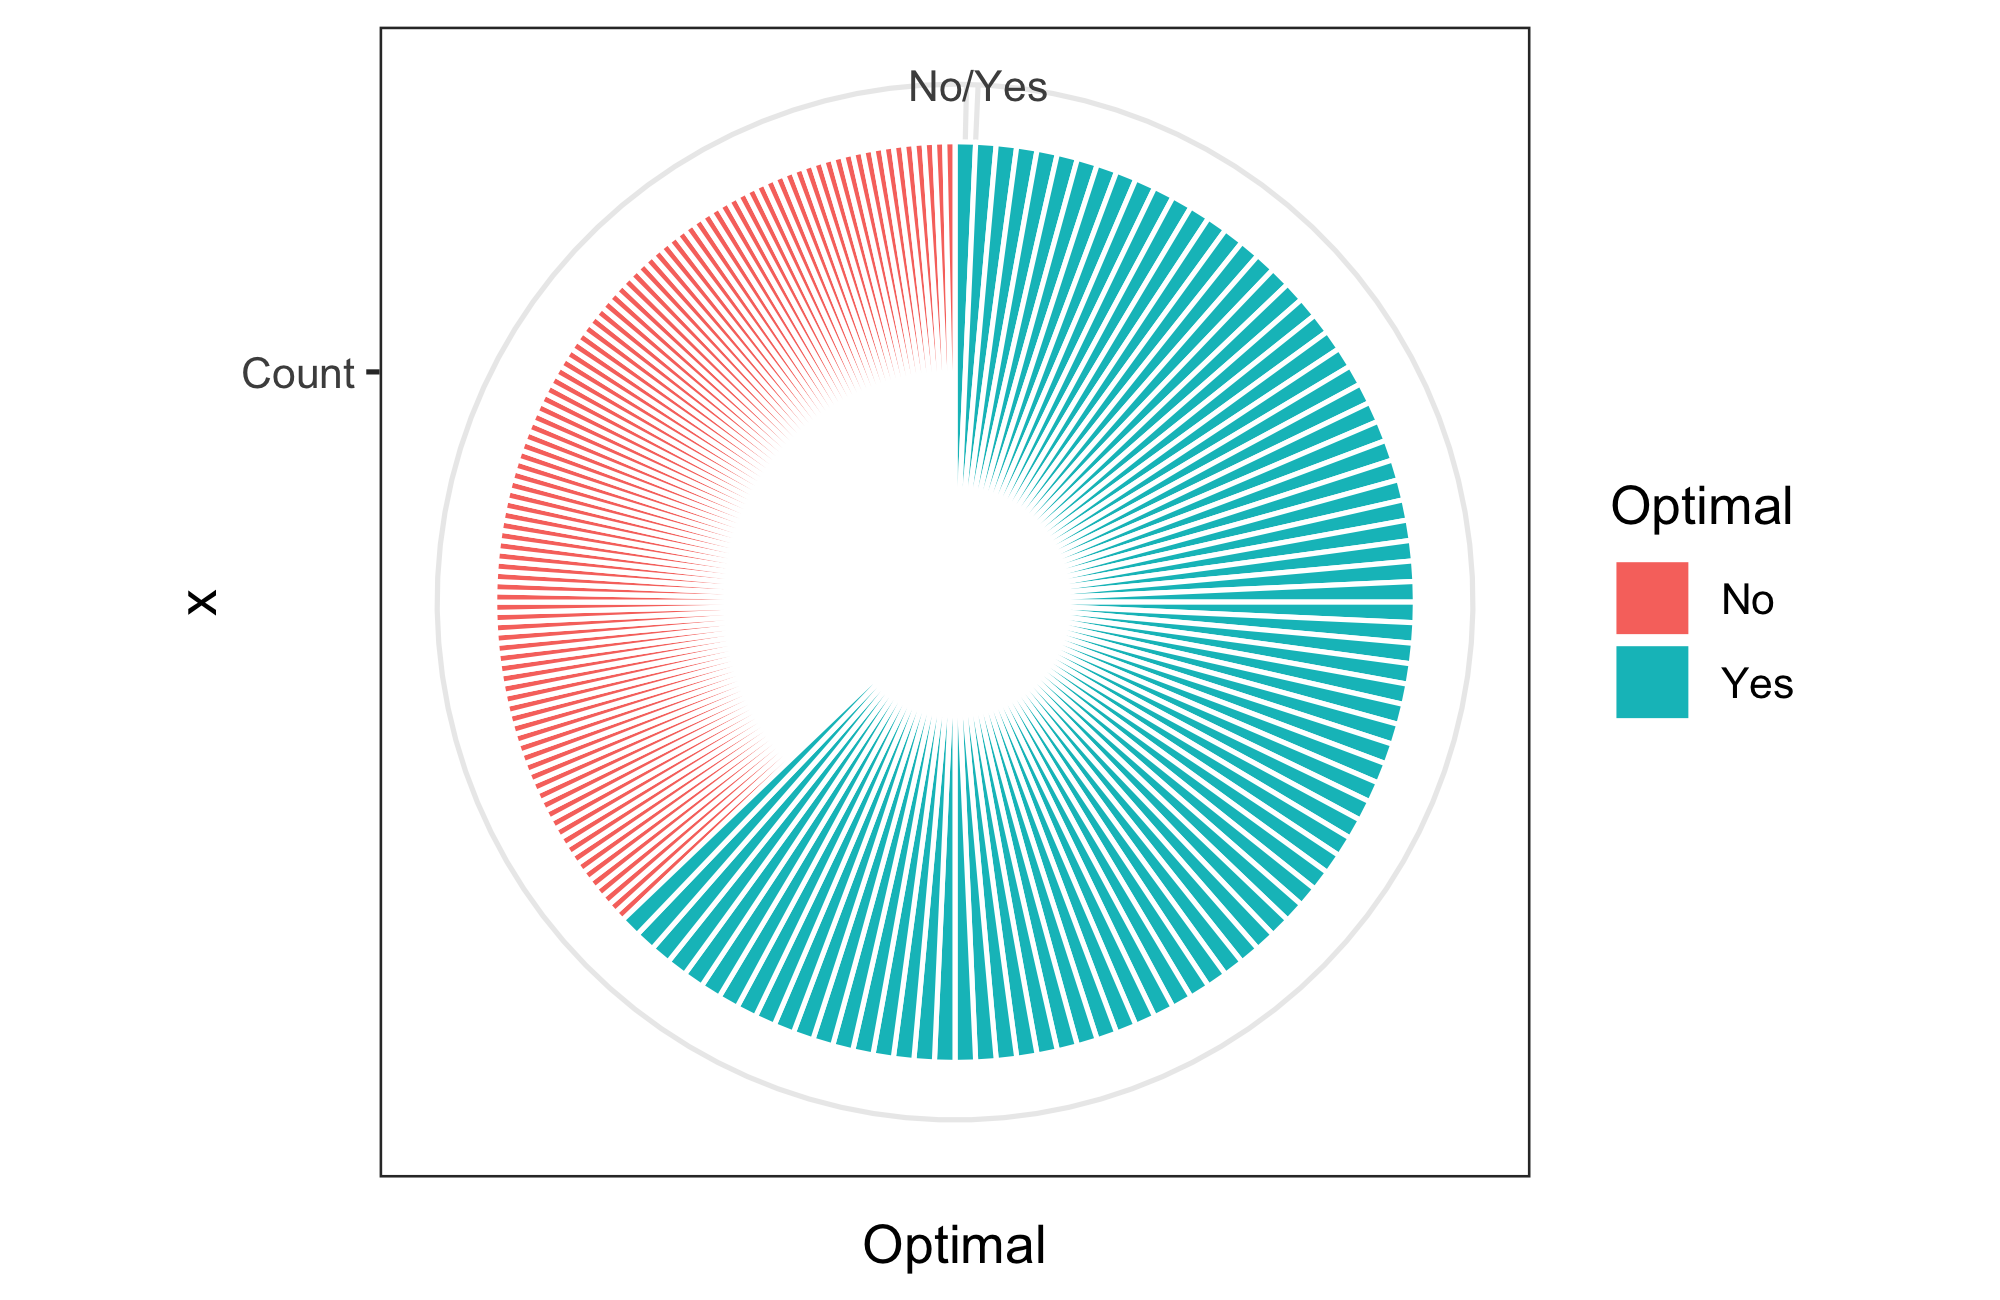
\includegraphics[width=\textwidth]{extras/pie_optimal}
				\caption[]%
				{{\small Instances that reached optimal values}}    
				\label{fig:pie:optimal}
			\end{subfigure}
			\hfill
			\caption[ ]
			{\small Pie Charts of Results} 
			\label{fig:pies}
		\end{figure}
	
 
 \vspace{1cm}
 \VerbatimInput{extras/ctable1.txt}
 
  \VerbatimInput{extras/chisq.txt}
  
   \VerbatimInput{extras/ctableexpected.txt}

\clearpage	
\section{Covariance}
Covariance provides a measure of the strength of correlation between two variables or more sets of variables. In the covariance matrix de $ C_{ij}$ element corresponds to the covariance of $ x_{i }$ and $ x_{j }$, whereas the element $ C_{ii} $ is the variance of $ x_{i} $. The following properties can also be recognized:
\begin{itemize}
	\item If COV$(x_{i},x_{j}) = 0$ then variables are uncorrelated,
	\item If COV$(x_{i},x_{j}) > 0$ then variables are positively correlated,
	\item If COV$(x_{i},x_{j}) < 0$ then variables are negativetily correlated.
\end{itemize}

For the experiments, data of the adjusted close price of the stock market are downloaded from the Yahoo Finance website, in the timeframe from January 2007 to March 2017, the chosen companies are Procter \& Gamble and its german peer Beiersdorf.

The first proof is that $\mbox{Cov}[aX+b, cY+d] = ac\mbox{Cov}[X,Y]$. For this experiment coefficients $a$, $b$, $c$, $d$ of different distributions are generated 30 times each, in order to have a certain grade of diversity. In all the iterations results were the same. The used code is shown below:

\lstinputlisting[language=R, firstline=8, lastline=22]{covariance.R}

The second proof is that $\mbox{Var}[X+Y] = \mbox{Var}[X] + \mbox{Var}[Y] + 2\mbox{Cov}[X,Y]$. For this experiment, the mentioned variances of the adjusted close prices are calculated, and then the values of both sides of the equation are compared. The result is confirmed with a value of 968.83. The used code is shown below:

\lstinputlisting[language=R, firstline=25, lastline=27]{covariance.R}

			
\clearpage

	\bibliography{a11}
	\bibliographystyle{plainnat}

\end{document}